\section{光传导}
\subsection{视杆中的光传导}
\begin{frame}
    \frametitle{视杆与视锥中的光传导}

    \begin{columns}
        \column{.5\textwidth}{
            在光感受器中,光对视色素的刺激激活G蛋白,然后激活一种效应器酶,
        改变胞内第二信使分子的浓度,从而导致膜上例子通道的关闭,膜电位因此改变。如图\ref{pic5-1}所示。
        }\column{.5\textwidth}{
            \begin{figure}
                \centering
                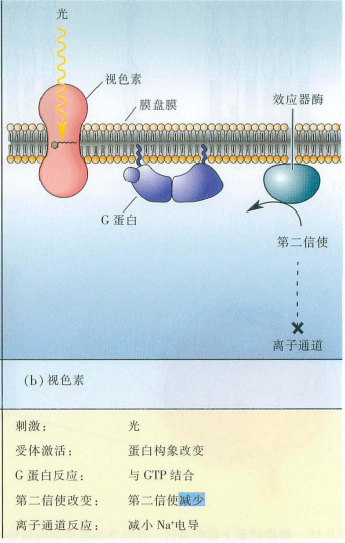
\includegraphics[height=.7\textheight]{img/pic5-1.png}
                \caption{视色素被激活的过程\label{pic5-1}}
            \end{figure}
        }
    \end{columns}

\end{frame}

\begin{frame}
    \frametitle{光感受器的膜电位变化过程}
    \begin{columns}
        \column{.5\textwidth}{
            神经元静息膜电位大约为$-65$mV,在完全黑暗的环境下,视杆外段的膜电位约为$-30$mV这个\textbf{去极化}是由$Na^+$的内流引起的,称为\textbf{暗电流}(dark current),
            钠离子通道是由称为\textbf{环鸟苷酸}(cGMP)的胞内第二信使开启,光照使得cGMP减少,导致钠离子通道关闭,膜电位更趋于负。于是光感受器对光反应呈\textbf{超极化}。
            
            对光感受器的持续光照使得cGMP水平降低,从而使对光反应达到饱和,进一步的光照不会引起更大程度的超极化。
        }\column{.5\textwidth}{
            \begin{figure}
                \centering
                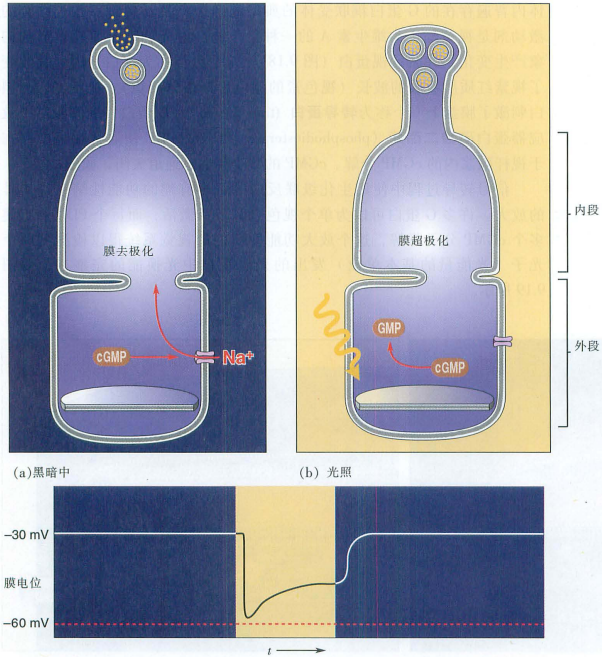
\includegraphics[height=.7\textheight]{img/pic5-2.png}
                \caption{光感受器对光反应的超极化\label{pic5-2}}
            \end{figure}
        }
    \end{columns}


\end{frame}
% #TODO:视杆中光感受器的具体生化反应过程
\subsection{视锥中的光传导}
\begin{frame}
    \frametitle{视锥中的光传导}

    白天的视觉完全依赖于视色素在不同视锥中的差异,视锥中的视色素需要更多的能量才能被漂白。
    视锥细胞互斥的拥有三种视蛋白(可被称为“红”锥、“绿”锥、“蓝”锥)使得视色素具有不同的光谱敏感性。
    三种视锥细胞不同程度的激活共同形成了我们认识到的色彩信号,而这个色觉理论被称为\textbf{Young-Helmholtz三原色理论}。
    \begin{figure}
        \centering
        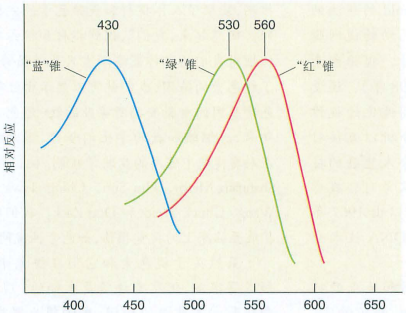
\includegraphics[height=.4\textheight]{img/pic5-3.png}
        \caption{三种视锥色素的光谱敏感性\label{pic5-3}}
    \end{figure}
\end{frame}

% #TODO:可以加一点计算机图形学的东西
\subsection{暗适应和明适应}
\begin{frame}
    \frametitle{暗适应和明适应}

    从全视锥的明视到全视杆的暗视约需要20\~25min的适应时间,该现象称为\textbf{暗适应}(dark adaptation)。在这个阶段中光的敏感性提升了100万倍,瞳孔放大,未漂白的视紫红质再生,视网膜功能贿赂的调节以使每个神经节细胞可以接受更多来自视杆的信息。

    从全视杆的暗视到全视锥的明视约需要5\~10min的适应时间,该现象称为\textbf{明适应}(light adaptation)。其过程基本与暗适应相反。

\end{frame}